\section{Introduction}
\begin{wrapfigure}{r}{0.3\textwidth}
	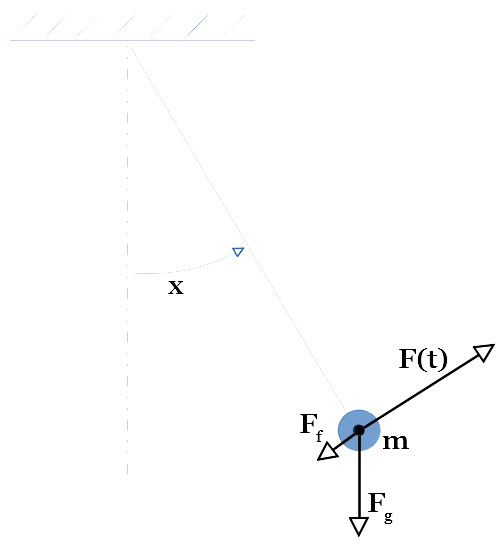
\includegraphics[width=0.25\textwidth]{figures/pendulum.png}
	\caption{Schematic drawing of basic pendulum subject to a driving, gravitational and a frictional force corresponding to the symbols $F(t)$, $F_g$ and $F_f$ respectively. $x$ corresponds to the excitation of the pendulum.}
	\label{fig_pendulum}
\end{wrapfigure}

From quantum effects to pendulums and from data exchange to clocks, there are many phenomena and devices that are governed by harmonic oscillators. Since harmonic oscillators can be used to describe any system with a smooth potential near a stable equilibrium and many corresponding applications, it is a popular topic in physics. The harmonic oscillator is defined as a system in subject to a restoring force that is proportional to the displacement from an equilibrium position. As a result of this restoring force, harmonic oscillators will describe an oscillatory motion. \\
The aim of this study is to give insights in the behaviour of different types of harmonic oscillators subject to driving forces. This could, for example, be useful for data exchange in quantum physics. \\
For this experiment we will take a look at a basic pendulum subject to a driving force and a frictional force such as in the schematic drawing in figure \ref{fig_pendulum}. With $x$, the angle of excitation, $m$ the mass of the pendulum, $F(t)$ the driving force, $F_f$ the friction force and $F_g$ the gravitational force on the mass. \\
We can solve $x(t)$ using Newtons second law of motion:

\begin{align*}
	m \: a = \sum F  \\
	m \ddot{x} = - F_{g,x} - F_f + F(t)
\end{align*}

To solve $x$ as function of $t$, we suppose $F_f$ is directly proportional to the velocity and note that the gravitational force in the $x$ direction is given by $F_{g,x} = - F_g \sin(x) = - m \: g \: \sin(x)$, with $g$ the gravitational constant.
\begin{align*}
	m \ddot{x} = - m \: g \: \sin(x) - \alpha \: \dot{x} + F(t)
\end{align*}

For small values of $x$ we can use a Taylor expansion for $\sin(x)$ which yields $\sin(x) \approx x$. Therefore, for small values of $x$ we get the following differential equation:
\begin{align*}
	m \ddot{x} + \alpha \: \dot{x} + m \: g \: x = F(t)
\end{align*}
When there would be no frictional or driving force we would get:
\begin{align*}
	m \ddot{x} + m \: g \: x = 0
\end{align*}
This is straight forward to solve and gives:
\begin{align*}
	x(t) = \beta_1 e^{i \omega t} + \beta_2 e^{-i \omega t}
\end{align*}
With $\beta_1$, $\beta_2$ two arbitrary constants that depend on the initial conditions and $\omega = \sqrt{g}$ the natural frequency of the pendulum. We also define $alpha =\frac{m \: \omega}{Q}$, with $Q$ the quality factor of the system. This would mean that for higher values of $Q$, the frictional force would be less and there would be fewer energy dissipation by the system. The $m$ and $\omega$ terms are necessary in this definition of $\alpha$ in order to make the term equal to a force. \\
Finally we find the following differential equation:
\begin{equation}
	m \ddot{x}(t) + m \frac{\omega}{Q} \dot{x}(t) + m \omega^2 x(t) = F(t)
	\label{eq_diff}
\end{equation}
In this report, the behaviour of a pendulum subject by three types of driving forces will be studied. This will be done for a pendulum with a conventional frictional force, one without friction and one with 'inverse' friction. This corresponds to the values of $Q=1$, $Q \rightarrow \infty$ and $Q=-1$ respectively.
In the first part of this report, we will study the behaviour of the driven oscillator for an infinite driving force of $F(t) = F_0 \cos{\omega t}$. This is solved analytically . In the second part, a finite excitation $F(t) = F_0 \cos(\omega t)$ for $0 < t < T$ and $F(t) = 0$ for $t \geq T$ with three different values $\omega T = 0.1$, $\omega T = 1$ and $\omega T = 10$ are solved analytically and studied. In the final part a finite driving force of $ F(t) = F_0 t\frac{T-t}{T^2}$ for the same values of $\omega T$ as in the previous section. \\








